%File: formatting-instruction.tex
\documentclass[letterpaper]{article}
\usepackage{url,graphicx,xcolor}
\usepackage{times}
\usepackage{helvet}
\usepackage{courier}
\usepackage[hidelinks]{hyperref}
\usepackage[
    % guidelines
]{faikrmod3}
\usepackage{booktabs}
\usepackage{multirow}
\usepackage{makecell}
\usepackage{array}
\usepackage{bookmark}
\usepackage{footnote}
\usepackage[nameinlink]{cleveref}
\usepackage[bottom]{footmisc}
\frenchspacing
\setlength{\pdfpagewidth}{8.5in}
\setlength{\pdfpageheight}{11in}


% THE \pdfinfo /Title AND /Author ARE NOT NECESSARY, THEY ARE METADATA FOR THE FINAL PDF FILE
\pdfinfo{
/Title (Comparing Structure Learning Algorithms Across Different Libraries)
/Author (Tian Cheng Xia)}
\setcounter{secnumdepth}{0}  
 \begin{document}
% The file aaai.sty is the style file for AAAI Press 
% proceedings, working notes, and technical reports.
%
\title{Comparing Structure Learning Algorithms Across Different Libraries}
\author{Tian Cheng Xia\\
Master's Degree in Artificial Intelligence, University of Bologna\\
tiancheng.xia@studio.unibo.it
}
\maketitle


\attention{DO NOT MODIFY THIS TEMPLATE - EXCEPT, OF COURSE FOR TITLE AND AUTHORS. REMOVE THE \texttt{guidelines} OPTION FROM  \texttt{$\backslash$usepackage[guidelines]\{faikrmod3\}} IN THE \LaTeX\ SOURCE IN THE FINAL VERSION.}

\begin{abstract}
\begin{quote}

This mini-project aims to explore and test the different structure learning algorithms available
in the existing open-source libraries for Bayesian networks.
We reviewed the available Python libraries and 
experimented with the algorithms available in four of them, evaluating the methods on classification tasks.
We empirically observed that networks learned using tree-based methods are less accurate but inherently simpler while
constraint-based and score-based methods are more accurate but result in more complex topologies.

\explanation{
This mini-project aims to ... \\
We use ... \\
We found that ...
}

\end{quote}
\end{abstract}


\section{Introduction}

\subsection{Domain}
Structure learning algorithms are methods to infer the topology of a Bayesian network through independence tests or fitness scores.
Various algorithms have been proposed in the literature and in this mini-project we explore what has been implemented in the existing Python libraries.

\explanation{
Introduce your work: what you are modeling, if you are drawing inspiration from an existing model, study, paper, textbook example, challenge, \dots.\\
Briefly provide whatever background information on the domain you think is necessary for the reader to understand the model and your design choices.
}
\attention{HERE AND EVERYWHERE ELSE: ALWAYS KEEP IN MIND THAT, CRUCIALLY, WHATEVER TEXT/CODE/FIGURES/IDEAS/... YOU TAKE FROM ELSEWHERE MUST BE CLEARLY IDENTIFIED AND PROPERLY REFERENCED IN THE REPORT.}


\subsection{Aim}
% In this mini-project, we aim to review and evaluate the structure learning algorithms available 
% in the existing open-source Python libraries for Bayesian networks.
In this mini-project, we aim to review existing open-source Python libraries that implement structure learning algorithms
and evaluate them on classification problems.

\explanation{
Explain the purpose of your project: what do you intend to observe/try/experience/\dots? \\
\begin{itemize}
% \item Example: the purpose of this project is to implement part of the Bayesian network described in \cite{10.1371/journal.pone.0220065} and experiment with concepts seen in class \\
\item Another example: our aim was to experiment the effect of discretization of continuous variables \\
\item Yet another example: we are interested in comparing the run-time and error of approximate inference under different conditions
\item One final example: we studied \textit{value of information}: something mentioned in class but not covered in this module, which sparked our interest.
\end{itemize}
}


\subsection{Method}
% We evaluate the available structure learning algorithms on the task of classification.
To train and test the available structure learning algorithms, 
we use the following datasets where continuous features have been discretized:
\begin{itemize}
    \item \textit{Apple quality}, with 7 Gaussian distributed features.
    \item \textit{Heart disease}, with 13 features, mostly categorical.
\end{itemize}

The libraries we experimented with are listed in \Cref{tab:libraries}.
Other libraries (\texttt{PyOpenPNL}, \texttt{pyBN}, \texttt{libpgm})
have been discarded as they are outdated and not actively maintained.

\begin{table}[h]
    \small
    \centering
    \begin{tabular}{cccc}
        \toprule
        \textbf{Library} & \textbf{Version} & \textbf{Backend} & \textbf{License}\\
        \midrule
        \texttt{pgmpy}          & 0.1.24    & Numpy             & MIT \\
        \texttt{bnlearn}        & 0.8.4     & \texttt{bnlearn}  & MIT \\
        \texttt{pomegranate}    & 1.0.3     & PyTorch           & MIT \\
        \texttt{pyAgrum}        & 1.11.0    & C++               & GPLv3 \\
        % \texttt{PyOpenPNL} & & & \\
        % \texttt{pyBN} & & & \\
        % \texttt{libpgm} & BSD-3 & 1.3 & Numpy \\
        % \texttt{LGNpy} & MIT & & Numpy \\
        \bottomrule
    \end{tabular}
    \caption{Overview of the experimented libraries.} 
    \label{tab:libraries}
\end{table}



\explanation{
Describe the methodology you followed
\begin{itemize}
    \item Example: we used pgmpy library methods\footnote{This is just an example: indeed, it is NOT necessary to use pgmpy; the coding language doesn't have to be python either. Feel free to use whatever software framework suits your needs.} to implement our network and run queries. To understand if differences in models, queries, parameters or number of samples induced differences in accuracy, we varied evidence nodes, conditional probability distributions, inference method, ...
\end{itemize}
}

\subsection{Results}

We empirically observed that among the various classes of structure learning algorithms, 
tree-based methods are less accurate but produce a smaller network while
constraint-based and score-based methods achieve higher accuracy at the cost of a more complex model.

\explanation{
In a few lines: what are the most noteworthy results you have observed or things you have learned/understood from this project? (only the highlights: there will be a dedicated paragraph for presenting results in the Analysis section)
}


\section{Model}

As we are interested in testing structure learning algorithms, 
we infer the topology of the networks using these methods and, 
for a more straightforward and fair comparison, we always use MLE as parameter learning algorithm and
make queries only using exact inference through variable elimination.
The algorithms available in each library we experimented with are listed in \Cref{tab:libraries_algos}.
When allowed, we tried different fitness functions and independence tests.

\begin{table*}[ht]
    \small
    \begin{minipage}{\textwidth}
        \renewcommand*\footnoterule{}
        \centering
        \begin{tabular}{ccccc}
            \toprule
            \multirow{2}{*}[-2pt]{\textbf{Library}} & \multicolumn{4}{c}{\textbf{Structure learning algorithms}} \\
            \cmidrule(r){2-5}
            & \multicolumn{1}{c}{\textbf{Score-based}} & \multicolumn{1}{c}{\textbf{Tree-based}} & 
                \multicolumn{1}{c}{\textbf{Constraint-based}} & \multicolumn{1}{c}{\textbf{Hybrid}} \\
            \midrule
            \makecell{\texttt{pgmpy}\\\texttt{bnlearn}} &
                \makecell{
                    Hill-climbing\\
                    Exhaustive search
                } & 
                \makecell{
                    Chow-Liu\\
                    Naive Bayes\\
                    Tree-augmented NB
                } & 
                \makecell{PC} &
                \makecell{Max-min hill-climbing} \\
            \midrule
            \texttt{pomegranate} &
                \makecell{A*\footnote{Not explicitly listed in the official documentation.\label{pomegranate_doc}}} & 
                \makecell{Chow-Liu\footref{pomegranate_doc}} & 
                \makecell{---} &
                \makecell{---} \\
            \midrule
            \texttt{pyAgrum} &
                \makecell{
                    Hill-climbing\\
                    Tabu search\\
                    K2
                } & 
                \makecell{
                    Chow-Liu\footnote{Only available for Bayesian network classifiers.\label{pyagrum_bnc}}\\
                    Naive Bayes\footref{pyagrum_bnc}\\
                    Tree-augmented NB\footref{pyagrum_bnc}
                } & 
                \makecell{MIIC} &
                \makecell{---} \\
            \bottomrule
        \end{tabular}
    \end{minipage}
    \caption{Structure learning algorithms available in each library.} 
    \label{tab:libraries_algos}
\end{table*}

% \explanation{
% Insert a picture of your Bayesian network(s) (Figure~\ref{fig:network})
% \begin{figure}
%     \centering
%     \includegraphics[scale=1.0]{F2.png}
%     \caption{Bayesian network. Image taken from \url{https://www.intechopen.com/chapters/62844}}
%     \label{fig:network}
% \end{figure}
% }

\explanation{
Explain the following aspects of your model (if there is too much to say and not enough space, put in your notebook whatever does not fit here):
\begin{itemize}
    \item nodes: if not self-explanatory, explain each random variable's meaning/intuition and type/range
    \item conditional distributions (for example, the CPTs, some or all of them)
    \item the procedure you followed to build your model (structure and conditional distributions): from reference paper? by analyzing the domain? learned from data? just assigned probability distributions arbitrarily? followed a particular methodology for building the network? ...
\end{itemize}  
In general, only write whatever is relevant and necessary to understand the rest of the report. Do not explain concepts seen in class or explained in textbooks. Do not describe models taken from textbook/literature/tutorials/libraries, like (for example) the Asia network. Instead, if you are using a model as-is: just insert a reference or URL\footnote{\url{https://www.bnlearn.com/bnrepository/}.}
}

\section{Analysis}

\subsection{Experimental setup}
Each dataset has been split into a train and test set.
The train set is fed to the structure learning algorithms to determine the topology of the network.
The test set is used to evaluate the resulting models by querying the target variable given as evidence the other features.

For each structure learning algorithm, we keep track of the classification metrics,
the time required to learn the structure, and the total number of edges in the computed model.

\explanation{
Briefly describe the probability queries or other experiments that you have carried out. Describe how you plan to evaluate the results (for example: are there results that you would expect?)
}

\subsection{Results}

Results on the \textit{apple quality} dataset are shown in \Cref{img:apple}.
The highest accuracy is achieved by two score-based algorithms: hill-climbing and tabu search
while tree-based methods are those that obtain the lowest accuracy.
On the other hand, analyzing the complexity of the learned network, intended as the number of edges,
we can observe that tree-based methods, as expected, produce simpler topologies, while A* and hill-climbing result in bigger models.

\begin{figure}[h]
    \centering
    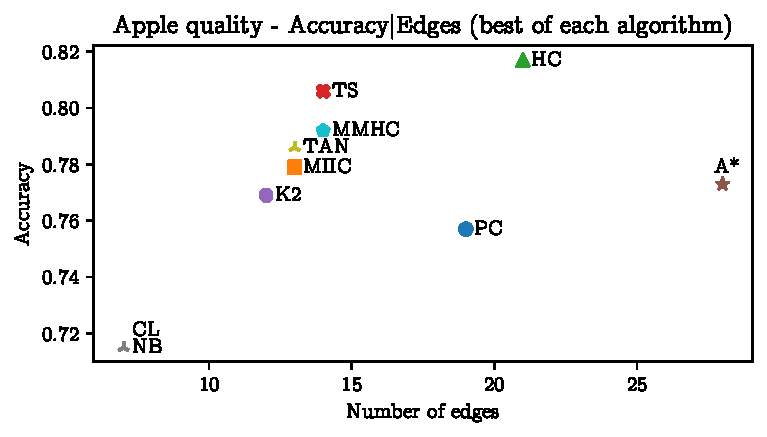
\includegraphics[width=\linewidth]{img/apple_acc_edges.pdf}
    \caption{Relationship between accuracy and number of edges on the \textit{apple quality} dataset.}
    \label{img:apple}
\end{figure}

Results\footnote{A* and MMHC have been omitted as they are computationally too expensive.} 
on the \textit{heart disease} dataset are presented in \Cref{img:heart}.
In this case, the PC algorithm reaches the highest accuracy while, again, tree-based methods obtain the lowest performance.
Hill-climbing is still one of the best-performing methods but 
it is also among the algorithms that result in the most complex topology.

\begin{figure}[h]
    \centering
    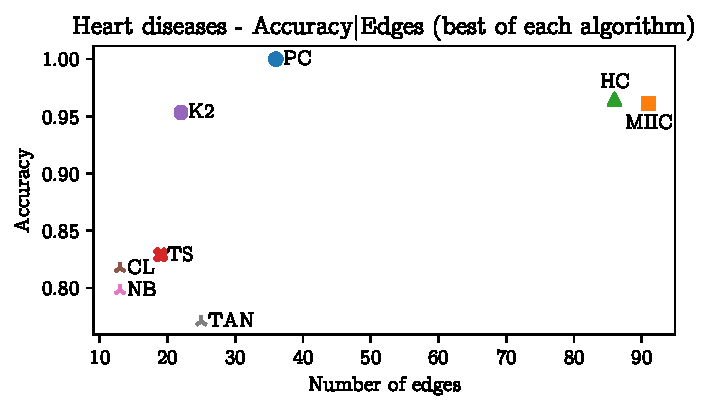
\includegraphics[width=\linewidth]{img/heart_acc_edges.pdf}
    \caption{Relationship between accuracy and number of edges on the \textit{heart disease} dataset.}
    \label{img:heart}
\end{figure}

Overall\footnote{For more details regarding our experiments, we refer the reader to the \texttt{plots.ipynb} notebook.}, 
we can empirically observe that hill-climbing is the most consistent algorithm
across the two datasets but lacks the capability of creating a simpler topology.
Tree-based methods are instead those with the lowest, but still acceptable, results and 
have the advantage of learning smaller and more interpretable networks.

Compared to the literature, our results are in line with what is observed in \cite{learning_comparison_2021}.
In fact, the performances of the various structure learning algorithms depend on the data and 
it is not possible to select one as the best.




\explanation{
What did you observe? \\
All according to expectations? \\
Anything surprising or worthwhile mentioning?
}


\section{Conclusion}

In this mini-project, we explored the structure learning algorithms available in four Python libraries.
We evaluated these algorithms on two classification datasets and 
empirically observed that it is not reasonable to label one of them as the best as it heavily depends on the data.
From a more general point of view, we concluded that tree-based methods produce less accurate but simpler networks
while constraint-based and score-based methods have higher accuracy but result in more complex topologies.
An interesting experiment we did not cover is to assess the capability of structure learning algorithms to recreate
a network given the data sampled from a known topology.

\explanation{
Just one paragraph: what you have learned, anything interesting that came up, what are the limitations of your model/experiments/study/...
}


\section{Links to external resources}

\begin{itemize}
    \item \textit{Apple quality} dataset: {\small\url{https://www.kaggle.com/datasets/nelgiriyewithana/apple-quality}}.
    \item \textit{Heart disease} dataset: {\small\url{https://www.kaggle.com/datasets/ineubytes/heart-disease-dataset}}.
\end{itemize}

\explanation{
Optionally, insert here:
\begin{itemize}
    \item a link to your GitHub or any other public repo where one can find your code (only if you did not submit your code on Virtuale) 
    \item a link to your dataset (only if you have used a dataset, for example, for learning network parameters or structure)
\end{itemize}
Leave this section empty if you have all your resources in Virtuale. \textbf{Do not insert code/outputs in this report}.
}
\bigskip

\bibliographystyle{aaai}
\bibliography{faikrmod3.bib}

\attention{NOTICE: THIS REPORT'S LENGTH MUST NOT EXCEED \textbf{TWO PAGES} PLUS REFERENCES. THIS MAY MEAN THAT YOU WILL HAVE TO LEAVE OUT OF THE REPORT PART OF THE WORK YOU HAVE DONE OR OBSERVATIONS YOU HAVE. THIS IS NORMAL: THE REPORT SHOULD EMPHASIZE WHAT IS MOST SIGNIFICANT, NOTEWORTHY, AND REFER TO THE NOTEBOOK FOR ANYTHING ELSE. FOR ANY OTHER ASPECT OF YOUR WORK THAT YOU WOULD LIKE TO EMPHASIZE BUT CANNOT EXPLAIN HERE FOR LACK OF SPACE, FEEL FREE TO ADD COMMENTS IN THE NOTEBOOK.}


\end{document}